%% ================================================================
\chapter{Chapter title}
\label{chap:one_chapter}

%% ----------------------------------------------------------------
\section{Disclaimers and usage instructions}

This is a version of my PhD dissertation which I defended and got through
Graduate College format review in spring 2010.  I hope it works for you.
Please keep in mind, however, that style policies may change.  Of course,
please consult the style information you received from the Graduate College.

I should acknowledge that I didn't write this from scratch.  I got this
template from I forget where --- somewhere in LPL, I think --- and modified to
my taste, and to match current formatting requirements.  So, this is a current
snapshot of collectively developed dissertation style for the University
of Arizona.

How to use this template:

\begin{itemize}

\item Search around in
\texttt{stu-dent-dis.tex},
\texttt{ua-thesis.cls},
\texttt{Acknowledgement.txt}, etc. for the names ``Stuart Dent'' and
``Anna Mehmbuhr'', etc.  Change these to your name and the names of your
committee members.  Also change the title of your dissertation.

\item In those same files, look for anything else which needs changing.

\item In the first line of \texttt{stu-dent-dis.tex}, you can set the style to
\texttt{draft} or \texttt{final}.

\item The shell scripts \texttt{./dbuild} and \texttt{./pbuild}, in the
same directory as this file, can be used to create DVI and PDF files,
respectively.

\item Any {\LaTeX} problem you have is most likely resolvable by a Google
search.

\item Good luck, and have fun!

\end{itemize}

--- John ``Stu Dent'' Kerl, April 21, 2010.

%% ----------------------------------------------------------------
\section{Section title}
\label{sec:a_section}

The quick brown \plainidx{fox} jumped over the lazy \plainidx{dogs}.
The quick brown fox jumped over the lazy dogs.
The quick brown fox jumped over the lazy dogs.
The quick brown fox jumped over the lazy dogs.
The quick brown fox jumped over the lazy dogs.
The quick brown fox jumped over the lazy dogs.
The quick brown fox jumped over the lazy dogs.
The quick brown fox jumped over the lazy dogs.
The quick brown fox jumped over the lazy dogs.
The quick brown fox jumped over the lazy dogs.
The quick brown fox jumped over the lazy dogs.
The quick brown \emphidx{fox} jumped over the lazy dogs.

Table \ref{table:quadratic_data} will be discussed in section
\ref{sec:another_section}.

\begin{table}[thb]
$$
\begin{tabular}{|c|c|}
\hline $x$ & $f(x)$ \\
\hline
\hline $0$   &  $0$ \\
\hline $1$   &  $1$ \\
\hline $2$   &  $4$ \\
\hline $3$   &  $9$ \\
\hline $4$   & $16$ \\
\hline $5$   & $25$ \\
\hline
\end{tabular}
$$
\caption[Short caption for the list of tables.]
	{Here is the long caption for the body of the document.  Note that it's OK
	for this to have many lines.  But the short caption for the list of tables
	should be short.  Hence the difference between square brackets and curly
	braces in the \texttt{caption} command in the {\LaTeX} code.  And, you
	guessed it --- this last sentence is here just to make this caption even
	longer.
	\label{table:quadratic_data}}
\end{table}

%% ----------------------------------------------------------------
\section{Section title}
\label{sec:another_section}

\begin{table}[thb]
$$
\begin{tabular}{|c|c|}
\hline $x$ & $g(x)$ \\
\hline
\hline $0$   &   $0$ \\
\hline $1$   &   $1$ \\
\hline $2$   &   $8$ \\
\hline $3$   &  $27$ \\
\hline $4$   &  $64$ \\
\hline $5$   & $125$ \\
\hline
\end{tabular}
$$
\caption
	{Here is another caption.
	\label{table:cubic_data}}
\end{table}

The quick brown fox jumped over the lazy dogs.
The quick brown fox jumped over the lazy dogs.
The quick brown \plainidx{fox} jumped over the lazy \plainidx{dogs}.
The quick brown fox jumped over the lazy dogs.
The quick brown fox jumped over the lazy dogs.
The quick brown fox jumped over the lazy dogs.
The quick brown fox jumped over the lazy dogs.
The quick brown fox jumped over the lazy dogs.
The quick brown fox jumped over the lazy dogs.
The quick brown fox jumped over the lazy dogs.
The quick brown fox jumped over the lazy dogs.
The quick brown fox jumped over the lazy dogs.
The quick brown fox jumped over the lazy dogs.
The quick brown fox jumped over the lazy dogs.

Compare table \ref{table:cubic_data} with table \ref{table:quadratic_data}
which was on page \pageref{table:quadratic_data}.  We conjecture, but
are unable to prove, a relationship between these tabular data and
the function of equation \eqref{eqn:conjecture}:
\begin{align}
\label{eqn:conjecture}
	y &= x^4 - x^2 + 1.
\end{align}

%% ================================================================
\chapter{Chapter title}
\label{chap:another_chapter}

The quick brown fox jumped over the lazy dogs.
The quick brown fox jumped over the lazy dogs.
The quick brown fox jumped over the lazy dogs.
The quick brown fox jumped over the lazy dogs.
The quick brown fox jumped over the lazy dogs.
The quick brown fox jumped over the lazy dogs.
The quick brown fox jumped over the lazy dogs.
The quick brown fox jumped over the lazy dogs.
The quick brown fox jumped over the lazy dogs.
The quick brown fox jumped over the lazy dogs.
The quick brown fox jumped over the lazy dogs.
The quick brown fox jumped over the lazy dogs.
The quick brown fox jumped over the lazy dogs.

Please see figure \ref{fig:important}.

\begin{figure}[!htb]
\begin{center}
\psfragscanon
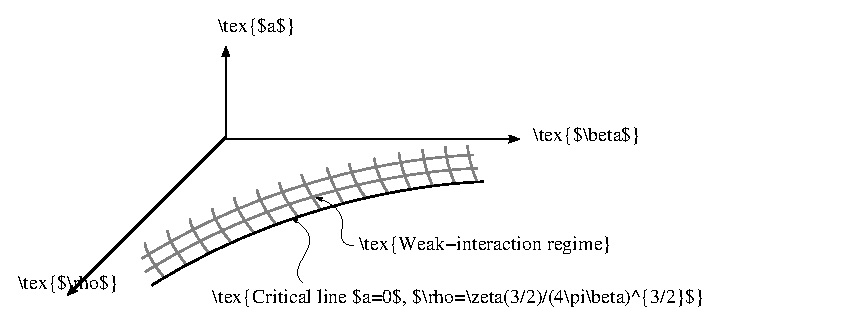
\includegraphics{figures/critical_manifold.eps}
\caption[Short caption for the list of figures.]
	{Here is an EPS file which I put in here and which surely must be
	important.
	\label{fig:important}}
\end{center}
\end{figure}

%% ----------------------------------------------------------------
\section{Section title}
\label{sec:yet_another_section}

The quick brown fox jumped over the lazy dogs.
The quick brown fox jumped over the lazy dogs.
The quick brown fox jumped over the lazy dogs.
The quick brown fox jumped over the lazy dogs.
The quick brown fox jumped over the lazy dogs.
The quick brown \emphidx{fox} jumped over the lazy \emphidx{dogs}.
The quick brown fox jumped over the lazy dogs.
The quick brown fox jumped over the lazy dogs.
The quick brown fox jumped over the lazy dogs.
The quick brown fox jumped over the lazy dogs.
The quick brown fox jumped over the lazy dogs.
The quick brown fox jumped over the lazy dogs.
The quick brown fox jumped over the lazy dogs.

%% ----------------------------------------------------------------
\section{Section title}
\label{sec:last_section}

The quick brown fox jumped over the lazy dogs.
The quick brown fox jumped over the lazy dogs.
The quick brown fox jumped over the lazy dogs.
The quick brown fox jumped over the lazy dogs.
The quick brown fox jumped over the lazy dogs.
The quick brown fox jumped over the lazy dogs.
The quick brown fox jumped over the lazy dogs.
The quick brown fox jumped over the lazy dogs.
The quick brown \plainidx{fox} jumped over the lazy \plainidx{dogs}.
The quick brown fox jumped over the lazy dogs.
The quick brown fox jumped over the lazy dogs.
The quick brown fox jumped over the lazy dogs.
The quick brown fox jumped over the lazy dogs.


\chapter{Chapter 3}
\label{chap: chapter3}
